%! Author = jordan
%! Date = 5/9/26

% Preamble
\documentclass[11pt]{article}
\title{AMATH 353 HW5}
\author{Jordan Tucker}
\date{May 9, 2026}

\renewcommand{\thesubsection}{(\alph{subsection})}
\makeatletter
\@addtoreset{subsection}{section}
\makeatother

% Packages
\usepackage{amsmath}
\usepackage{parskip}
\usepackage{tabularx}
\usepackage{graphicx}
\usepackage{enumitem}
\usepackage{amsthm}
\usepackage{amsfonts}
\usepackage{hyperref} %LaTeX package to import graphics
\graphicspath{{images/}} %configuring the graphicx package
\DeclareMathOperator{\sech}{sech}

% Document
\begin{document}
    \section*{Problem 1 - Fourier Series}
    Compute the coefficients $a_n,b_n$ in the Fourier series representations of each of the
    following functions.
    Then, determine the $x$ at which the series representations fail, if any.
    \begin{align*}
        a_n &= \frac{1}{L} \int_{-L}^{L} f(x) \sin(\frac{n \pi}{L} x) \,dx \\
        b_n &= \frac{1}{L} \int_{-L}^{L} f(x) \cos(\frac{n \pi}{L} x) \,dx
    \end{align*}

    \subsection{$f(x)=1+\cos(x) - \sin(2x) \quad L = \pi$}
    \begin{align*}
        \tilde f(x) &= \frac{b_0}{2} + \sum_{n=1}^\infty a_n \sin(nx) + b_n \cos(nx)\\
        1+\cos(x) - \sin(2x) &= \frac{b_0}{2} + \sum_{n=1}^\infty a_n \sin(nx) + b_n \cos(nx)\\
    \end{align*}
    By inspection:
    \begin{align*}
        &\frac{b_0}{2} = 1 \implies {b_0 = 2}\\
        &b_1 = 1, \quad b_n = 0 \ \text{for} \ n \neq 1\\
        &a_2 = -1, \quad a_n = 0 \ \text{for} \ n \neq 2\\
    \end{align*}
    Since $f(x)=1+\cos(x) - \sin(2x)$ is smooth and continuous, it's fourier series representation
    does not fail for any $x$.

    \subsection{$f(x)=x, \quad L = \pi$}
    Solving for $a_n$ and $b_n$ using formulas from class.

    \begin{align*}
        a_n &= \frac{1}{\pi} \int_{-\pi}^{\pi} x \sin(nx) \,dx \\
    \end{align*}
    Integration by parts (table method):

    \renewcommand{\arraystretch}{1.5}
    \begin{tabular}{ |c| c| }
        \hline
        $x$ & $\sin(nx)$ \\
        $-1$ & $-\frac{1}{n} \cos(nx)$ \\
        $0$ & $-\frac{1}{n^2} \sin(nx)$ \\
        \hline
    \end{tabular}

    \begin{align*}
        a_n \pi &=  -\frac{x}{n} \cos(nx) + \frac{1}{n^2} \sin(nx) \Big|_{-\pi}^{\pi} \\
        a_n \pi &= -\frac{\pi}{n} \cos(n \pi) + \frac{1}{n^2} \sin(n\pi) - \left( -\frac{-\pi}{n} \cos(-n \pi) + \frac{1}{n^2} \sin(-n\pi) \right)\\
        a_n \pi &= -\frac{\pi}{n} \cos(n \pi)  - \left( -\frac{-\pi}{n} \cos(- n \pi) \right)\\
        a_n &= -\frac{1}{n} \cos(n \pi)  - \left( -\frac{-1}{n} \cos(- n \pi) \right)\\
        a_n &= -\frac{1}{n} \cos(n \pi)  - \left( \frac{1}{n} \cos(- n \pi) \right) \quad \text{$\cos(n\pi) = \cos(-n\pi) = (-1)^n$}\\
        a_n &= -\frac{1}{n} (-1)^n - \left( \frac{1}{n}  (-1)^n \right) \\
        a_n &= -\frac{2}{n} (-1)^n\\
    \end{align*}
    Since $f(x) = x$ is an odd function, and $\cos(nx)$ is an even function, $f(x)\cos(nx)$ is an
    odd function.
    The integral
    $b_n &= \frac{1}{\pi} \int_{-\pi}^{\pi} x \cos(\frac{n \pi}{\pi} x) \,dx$ would be 0 since it is
    and odd function integrated over symmetric bounds.
    Therefor $b_n=0 \ \forall \ n  \in  \mathbb{Z}^+$

    The series fails at $x=\pi$ and $x = -\pi$ because of the jump discontinuities that exist there.

    \subsection{$f(x)=e^x, \ L = \pi$}

    Using the formula for $a_n$:
    \begin{align*}
        a_n = \frac{1}{\pi} \int_{-\pi}^{\pi} e^x \sin(n \pi) \,dx \\
    \end{align*}
    Using integration by parts with $u=\sin(nx)$, $du = n\cos(nx)$, $dv=e^x$, $v=e^x$
    \begin{align*}
        \int_{-\pi}^{\pi} e^x \sin(n \pi) \,dx &= \sin(nx)e^x - n \int e^x \cos(nx)  \\
    \end{align*}
    Using integration by parts again with $u=\cos(nx)$, $du = -n\sin(nx)$, $dv=e^x$, $v=e^x$
    \begin{align*}
        \int_{-\pi}^{\pi} e^x \sin(n \pi) \,dx &= \sin(nx)e^x - n \left( \cos(nx)e^x + n \int e^x \sin(nx) \,dx \right)  \\
        \int_{-\pi}^{\pi} e^x \sin(n \pi) \,dx &= \sin(nx)e^x - n \cos(nx)e^x - n^2 \int e^x \sin(nx) \,dx   \\
        \int_{-\pi}^{\pi} e^x \sin(n \pi) \,dx + n^2 \int_{-\pi}^{\pi} e^x \sin(nx) \,dx \right) ,\dx &= \sin(nx)e^x - n \cos(nx)e^x \Big|_{-\pi}^{\pi} \\
        \int_{-\pi}^{\pi} e^x \sin(n \pi) \,dx (1 + n^2)  &= \sin(nx)e^x - n \cos(nx)e^x \Big|_{-\pi}^{\pi}\\
        \int_{-\pi}^{\pi} e^x \sin(n \pi) \,dx &= \frac{\sin(nx)e^x - n \cos(nx)e^x}{1 + n^2} \Big|_{-\pi}^{\pi}
    \end{align*}
    We know that $\cos(n \pi) = \cos(-n\pi) = (-1)^n $
    \begin{align*}
        \int_{-\pi}^{\pi} e^x \sin(n \pi) \,dx &= \frac{-n(-1)^n e^{\pi}}{1+n^2} + \frac{n(-1)^n e^{-\pi}}{1+n^2}\\
        \int_{-\pi}^{\pi} e^x \sin(n \pi) \,dx &= \frac{-n(-1)^n}{1+n^2} (e^{\pi} - e^{-\pi}) \\
        a_n & = \frac{-n(-1)^n}{1+n^2 (\pi)} (e^{\pi} - e^{-\pi})
    \end{align*}

    For $b_n$, we can also use the formula:
    \[
        b_n = \frac{1}{\pi} \int_{-\pi}^{\pi} e^x \cos(nx) \,dx
    \]
    Using integration by parts, with $u=\cos(nx)$, $du = -n\sin(nx)$, $v=e^x$, $dv=e^x$.

    \begin{align*}
        \int_{-\pi}^{\pi} e^x \cos(nx) \,dx &= e^x \cos(nx) + n \int e^x \sin(nx)
    \end{align*}

    Using integration by parts again with $u=\sin(nx)$, $du=-n\cos(nx)$, $v=e^x$, $dv=e^x$.
    \begin{align*}
        \int_{-\pi}^{\pi} e^x \cos(nx) \,dx &= e^x \cos(nx) + n \sin(nx) - n^2 \int e^x \cos(nx)\\
        \int_{-\pi}^{\pi} e^x \cos(nx) \,dx +  n^2 \int_{-\pi}^{\pi} e^x \cos(nx) \,dx &= e^x \cos(nx) + n \sin(nx) \Big|_{-\pi}^{\pi} \\
        \int_{-\pi}^{\pi} e^x \cos(nx) \,dx (1+n^2) &= e^x \cos(nx) + n \sin(nx) \Big|_{-\pi}^{\pi}\\
        \int_{-\pi}^{\pi} e^x \cos(nx) \,dx &= \frac{ e^x \cos(nx) + n \sin(nx)}{1+n^2} \Big|_{-\pi}^{\pi}\\
        \int_{-\pi}^{\pi} e^x \cos(nx) \,dx &= \frac{e^{\pi}  \cos(n \pi)}{1+n^2} - \frac{e^{-\pi}  \cos(-n \pi)}{1+n^2}\\
        \int_{-\pi}^{\pi} e^x \cos(nx) \,dx &= \frac{e^{\pi}  (-1)^n}{1+n^2} - \frac{e^{-\pi} (-1)^n}{1+n^2}\\
        \int_{-\pi}^{\pi} e^x \cos(nx) \,dx &= \frac{(-1)^n}{1+n^2} (e^{\pi} - e^{-\pi})\\
        b_n &= \frac{1}{\pi}\frac{(-1)^n}{1+n^2} (e^{\pi} - e^{-\pi})
    \end{align*}
    The series fails at $x=\pi$ and $x = -\pi$ because of the jump discontinuities that exist there.

    \subsection{
        $f(x)=
        \begin{cases}
            0, & -\pi \le x \le 0, \\
            1-\dfrac{x}{\pi}, & 0 < x \le \pi
        \end{cases},
        \quad L=\pi$
    }

    Since the function is $0$ on the interval $-\pi \le x \le 0$, our bounds for our integrals only
    have to go from $0$ to $\pi$.

    For $b_0$:
    \begin{align*}
        b_n &= \frac{1}{\pi} \int_0^{\pi} (1-\frac{x}{n}) \,dx\\
        &=  \frac{1}{\pi} \left[ x-\frac{x^2}{2\pi} \Big|_0^{\pi} \right]\\
        &= \frac{1}{\pi} \left[ \pi - \frac{\pi^2}{2\pi} \right] \\
        b_0 &= 1 - \frac{1}{2} = \frac{1}{2}
    \end{align*}

    For $a_n$:
    \[
        a_n = \int_0^{\pi} (1-\frac{x}{\pi}) \sin(nx) \,dx
    \]
    Integration by parts using the table method:
    \begin{tabular}{ |c| c| }
        \hline
        $1-\frac{x}{\pi}$ & $\sin(nx)$ \\
        $\frac{1}{\pi}$ & $-\frac{1}{n} \cos(nx)$ \\
        $0$ & $-\frac{1}{n^2} \sin(nx)$ \\
        \hline
    \end{tabular}
    \begin{align*}
        a_n &= \frac{1}{\pi} \left[-(1-\frac{x}{\pi})\frac{1}{n} \cos(nx) - \frac{1}{\pi n^2}\sin(nx)  \right]_0^{\pi}\\
        &= 0 - (\frac{-1}{n \pi})
        a_n &= \frac{1}{n \pi}
    \end{align*}

    For $b_n$:
    \[
        b_n = \frac{1}{\pi} \int_{0}^{\pi} (1-\frac{x}{\pi}) \cos(nx) \,dx
    \]
    We can use integration by parts with the table method again:

    \begin{tabular}{ |c| c| }
        \hline
        $1-\frac{x}{\pi}$ & $\cos(nx)$ \\
        $\frac{1}{\pi}$ & $\frac{1}{n} \sin(nx)$ \\
        $0$ & $-\frac{1}{n^2} \cos(nx)$ \\
        \hline
    \end{tabular}

    \begin{align*}
        b_n &= \frac{1}{\pi} \left[ (1-\frac{x}{\pi})\frac{1}{n} \sin(nx) - \frac{1}{\pi n^2}\cos(nx) \right]_0^{\pi}\\
        &= \frac{1}{\pi} \left[ - \frac{-1^n}{n^2\pi} + \frac{1}{n^2 \pi} \right]\\
        b_n &= \frac{1-(-1)^n}{\pi^2 n^2}
    \end{align*}

    The series fails at $x=0$ due to the jump discontinuity that exits there.

    \newpage
    \section*{Problem 2 - Another Separation of Variables IBVP}
    Solve the finite-interval, \textbf{free-endpoint} wave equation IBVP given by
    \setcounter{subsection}{0}
    \subsection{Solve}

    \begin{gather*}
        \begin{cases}
            u_{tt}=c^2u_{xx}, & x\in [0,3], t\ge 0, \\
            u_x(0,t)=0, & t\ge 0, \\
            u_x(3,t)=0, & t\ge 0, \\
            u(x,0)=\cos^4(\frac{2}{3}\pi x), &  x \in [0,3],\\
            u_t(x,0)=0, & x \in [0,3].
        \end{cases}\\\\
        u_x(0,t) = u_x(3t) = 0\\\\
        u(x,t) = \frac{b_0}{2}+\sum_{n=1}^{\infty} b_n \cos(\frac{n\pi}{3}x) \cos(\frac{cn\pi}{3}t)\\
        u(x,0) = \cos^4(\frac{2}{3}\pi x)\\
        \text{Let $\theta = \frac{2}{3}\pi x$}\\
        \cos^4(\theta) = (\cos^2(\theta))^2 = \left(\frac{1}{2} (1+\cos(2\theta)) \right)^2
        \frac{1}{4}(1+2\cos(2\theta)+\cos^2(2\theta))\\
        \frac{1}{4}(1+2\cos(2\theta)+\frac{1}{2}+\frac{1}{2}\cos(4\theta))\\
        \frac{3}{8}+\frac{1}{2}\cos(2\theta)+\frac{1}{8}\cos(4\theta)\\
        u(x,0) = \frac{3}{8}+\frac{1}{2}\cos(\frac{4}{3} \pi x) + \frac{1}{8}\cos(\frac{8}{3} \pi x)\\
    \end{gather*}
    From inspection, we can see that:
    \begin{gather*}
        n=4,\ b_4 = \frac{1}{2}\\
        n=8,\ b_8 = \frac{1}{8}\\
        n=0,\ b_0 = \frac{3}{4}\\
    \end{gather*}
    So the final equation is:
    \[
        u(x,t) = \frac{3}{8} + \frac{1}{2}\cos\left(\frac{4\pi}{3}x\right)\cos\left(\frac{4c\pi}{3}t\right) + \frac{1}{8}\cos\left(\frac{8\pi}{3}x\right)\cos\left(\frac{8c\pi}{3}t\right)
    \]

    \subsection{Plot}

    \begin{figure}[h]
        \centering
        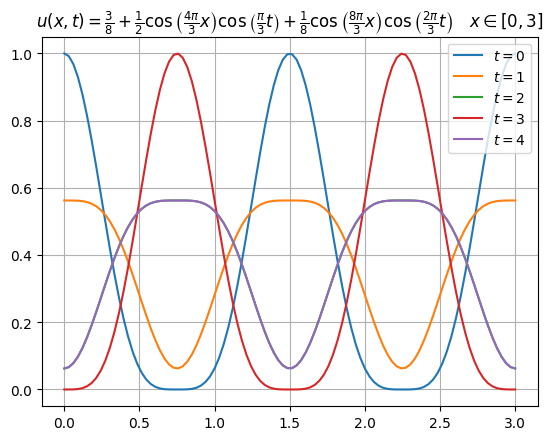
\includegraphics[width=0.75\textwidth]{hw5chart}
    \end{figure}
    
    \newpage
    
    \section*{Problem 3 - Laplace's Equation in Polar Coordinates}
    \setcounter{subsection}{0}
    Laplace's equation, $\Delta u = \nabla \cdot \nabla u = 0$, appears in a huge variety of applications, including but
    not limited to fluid mechanics, finance, electrostatics, heat conduction, image processing, and acoustics.
    In polar coordinates, it is given by
    \[
        u_{rr} + \frac{1}{r}u_r + \frac{1}{r^2}u_{\theta \theta}=0,
    \]
    \subsection{Use the separation of variables ansatz and derive the corresponding pair of ODEs}

    The ansatz is $u(r,\theta) = R(r) \Theta(\theta)$.

    Calculating the partial derivatives:
    \begin{gather*}
        u_r = R'(r) \Theta(\theta) \\
        u_{rr} = R''(r) \Theta(\theta)\\
        u_{\theta \theta} = R(r) \Theta''(\theta)
    \end{gather*}
    Plugging back into $u_{rr} + \frac{1}{r}u_r + \frac{1}{r^2}u_{\theta \theta}=0$:
    \begin{gather*}
        R''(r) \Theta(\theta) + \frac{1}{r} R'(r)\Theta(\theta) + \frac{1}{r^2} R(r)\Theta''(\theta) = 0\\\\
        \text{Multiply by original ansatz $R(r)\Theta(\theta)$}\\
        \frac{R''(r)}{R(r)} + \frac{R'(r)}{rR(r)} + \frac{\Theta''(\theta)}{r^2\Theta(\theta)} = 0 \\\\
        \text{Multiply by $r^2$}\\
        \frac{r^2R''}{R} + \frac{rR'}{R} + \frac{\Theta''}{\Theta} = 0 \\\\
    \end{gather*}
    Separate.
    Since one side depends only on $\theta$ and the other only on $r$, they must equal some
    constant $\lambda$
    \[
        \frac{r^2R''+rR'}{R}=-\frac{\Theta''}{\theta} = \lambda
    \]

    Simplify into two ODEs:
    \begin{gather*}
        \Theta'' + \lambda \Theta = 0\\
        r^2 R'' + rR' - \lambda R = 0
    \end{gather*}

    \subsection{Solve the ODEs}
    \begin{gather*}
        \Theta'' + \lambda \Theta = 0\\
        r^2 R'' + rR' - \lambda R = 0
    \end{gather*}

    Starting with $\Theta'' + \lambda \Theta = 0$.
    Since $\Tehta$ is $2\pi$ periodic, the following conditions apply:
    \begin{gather*}
        \Theta(\theta) = \Theta(\theta + 2\pi)\\
        \lambda = n^2,\ n=1,2,3,\dots
    \end{gather*}
    
    \textbf{Case $\lambda=0$}

    \begin{gather*}
        \Theta'' = 0\\
        \text{Integrating twice}\\
        \Theta = A_0 + B_0\theta\\
        \text{$B_0=0$ since it is periodic, it is not allowed to grow. So:}\\
        \Theta(\theta) = A_0
    \end{gather*}
    \textbf{Case $\lambda > 0, \ \lambda = n^2$}
    \begin{gather*}
        \Theta'' + n^2\Theta = 0\\
        \text{Harmonic Oscilator}\\
        \Theta = B_n\cos(n\theta) + A_n\sin(n\theta)
    \end{gather*}

    Solving $r^2 R'' + rR' - n^2 R =0$ next using cauchy euler:
    \begin{gather*}
        R(r) = r^{\alpha}\\
        R'(r) = \alpha r^{\alpha -1}\\
        R'' = \alpha(\alpha -1) r ^{\alpha-2}
    \end{gather*}
    Substituting back into our ODE:
    \begin{gather*}
        r^2 R'' + rR' - n^2 R = 0\\
        r^2 (\alpha(\alpha -1) r ^{\alpha-2}) + r\alpha r^{\alpha -1} - n^2 r^{\alpha} = 0\\
        (\alpha^2 - n^2) = 0 \implies \alpha=\pm n
    \end{gather*}

    \textbf{Case $n=0$. (repeated root $\alpha=0$)}
    \begin{gather*}
        R_0(r) = C_0 + D_0 ln(r)
    \end{gather*}
    \textbf{Case $n>0$. (two roots, $\alpha = n$ and $\alpha = -n)$}
    \[
        R_n(r) = C_n r^n + D_n r^{-n}
    \]

    Final ODE solutions:
    \begin{gather*}
        \Theta = B_n\cos(n\theta) + A_n\sin(n\theta)\\
        R_n(r) = C_n r^n + D_n r^{-n}
    \end{gather*}

    \subsection{Solve the boundary-value problem}
    \[
        \begin{cases}
            u_{rr} + \frac{1}{r}u_r + \frac{1}{r^2}u_{\theta \theta}=0, & 0 \le r \le R, 0 \le \theta \le 2\pi,\\
            u(R,\theta) = \cos(\theta)\sin(\theta), & 0 \le \theta < 2\pi\\
            u(r,2\pi) = u(r,0), & 0 \le r < R.\\
            \lim_{r\rightarrow0}|u(r,\theta)| < +\infty, & 0 \le \theta < 2\pi.
        \end{cases}
    \]
    \textit{The 3rd and 4th constraints effectively state that the angular component is 2$\pi$ periodic and that $u$ is bounded. Both of these conditions are necessary for the solution to be physical!}

    \begin{gather*}
        \Theta = B_n\cos(n\theta) + A_n\sin(n\theta)\\
        R_n(r) = C_n r^n + D_n r^{-n}
    \end{gather*}

    Because $\lim_{r\rightarrow0}|u(r,\theta)| < +\infty$, $r^{-n} = \frac{1}{r^n} \rightarrow \infty$ as $r \rightarrow 0$, so we need to get
    rid of that term in our second ODE by setting $D_0 = 0$, $D_n = 0$.

    \begin{gather*}
        \Theta = B_n\cos(n\theta) + A_n\sin(n\theta)\\
        R_0(r) = C_0\\
        R_n(r) = C_n r^n
    \end{gather*}

    Now we can multiply our ODES together to get the general solution.
    \begin{gather*}
        u(r,\theta) = \frac{b_0}{2} + \sum_{n=1}^{\infty} r^n (b_n \cos(n\theta) + a_n \sin(n \theta))
    \end{gather*}

    We can apply the initial condition $u(R,\theta) = \cos(\theta) \sin(\theta)$
    \begin{gather*}
        \frac{b_0}{2} + \sum_{n=1}^{\infty} R^n (b_n \cos(n\theta) + a_n \sin(n \theta) )= \cos(\theta) \sin(\theta)\\
        \frac{b_0}{2} + \sum_{n=1}^{\infty} R^n (b_n \cos(n\theta) + a_n \sin(n \theta) )= \frac{1}{2}\sin(2\theta)\\
        \text{By inspection:}\\
        \frac{b_0}{2} = 0 \implies b_0 = 0\\
        \text{No $\cos$ terms} \implies b_n =0\\
        a_2 R^2 = \frac{1}{2} \implies a_2 = \frac{1}{2R^2}
    \end{gather*}
    \textbf{Final solution after subbing back into the general solution at $n=2$}
    \[
        u(r,\theta) = \frac{r^2}{2R^2} \sin(2\theta)
    \]
    \newpage
    \section*{Problem 4 - Operators and Inner products}
    \setcounter{subsection}{0}
    \subsection{Show that $\left<u,v\right>_{L^2}$ defines an inner product.}
    \textbf{1. Symmetry}

    Since multiplication is commutative:
    \begin{gather*}
        \left<u,v\right>_{L^2} = \int_{-1}^{1} u(x)v(x)\,dx = \int_{-1}^{1} v(x)u(x)\,dx = \left<u,v\right>_{L^2}
    \end{gather*}
    So it is symmetrical.

    \textbf{2. Linearity}

    \begin{align*}
        \left<au+bv,w\right>_{L^2} &= \int_{-1}^{1} (au(x)+bv(x)) w(x) \,dx\\
        &= \int_{-1}^{1} au(x)w(x)+bv(x)w(x) \,dx\\
        &= \int_{-1}^{1} au(x)w(x) \,dx + \int_{-1}^{1} bv(x)w(x) \,dx\\
        \left<au+bv,w\right>_{L^2} &= a\left<u,w\right>_{L^2}+ b \left<v,w\right>_{L^2}
    \end{align*}
    Thus, $\left<u,v\right>_{L^2}$ is linear.

    \textbf{3. Positive definiteness}

    Let $u \in C_0^2([-1,1],\mathbb R)$ where $u\neq0$:

    \begin{align*}
        \left<u+,u\right>_{L^2} &= \int_{-1}^{1} u(x)u(x) \,dx\\
        &=\int_{-1}^{1} u(x)^2 \,dx\\
    \end{align*}
    $u(x)^2$ is always $> 0$ so its integral from $-1$ to $1$ will also be $>0$, thus $\left<u+,u\right>_{L^2}$
    is strictly positive.

    \subsection{Show that $\mathcal{L}=\partial_x^2$ is self-adjoint with respect to $\left<\cdot, \cdot\right>_{L^2}$
        on $C_0^2([-1,1],\R)$.}


    \begin{align*}
        \left<\mathcal{L}u,v\right>_{L^2} &= \int_{-1}^{1} \partial_x^2 u(x) v(x) \,dx \\
        &= \int_{-1}^{1} u''(x) v(x) \,dx
    \end{align*}
    Using integration by parts with $w=v(x)$, $dw=v'(x)$, $dz=u''(x)$, $z=u'(x)$
    \begin{align*}
        \left<\mathcal{L}u,v\right>_{L^2} &= u'(x)v(x)\Big|_{-1}^{1} - \int_{-1}^{1} u'(x)v'(x) \,dx
    \end{align*}
    Since $u,v \in C_0^2([-1,1],\mathbb{R})$, we know $v(1)=v(-1)=0$, so the boundary evaluates to 0.
    \begin{align*}
        \left<\mathcal{L}u,v\right>_{L^2} &= - \int_{-1}^{1} u'(x)v'(x) \,dx
    \end{align*}
    Using integration by parts again with $w=u'(x)$, $dw=u''(x)$, $dz=v'(x)$, $z=v(x)$:
    \begin{align*}
        \left<\mathcal{L}u,v\right>_{L^2} &= - \left( u(x)v'(x)\Big|_{-1}^{1} - \int_{-1}^{1} u(x)v''(x) \,dx \right)
    \end{align*}
    $u(1)=u(-1)=0$ so the boundary evaluates to 0
    \begin{align*}
        \left<\mathcal{L}u,v\right>_{L^2} &= \int_{-1}^{1} u(x)v''(x) \,dx \\
        &= \int_{-1}^{1} u(x)\partial_x^2v(x) \,dx \\
        \left<\mathcal{L}u,v\right>_{L^2} &= \left<u,\mathcal{L}v\right>_{L^2}
    \end{align*}
    Thus, $\mathcal{L}=\partial_x^2$ is self-adjoint.

    \subsection{Show that the eigenvalues of a self-adjoint operator are purely real and that the eigenvectors corresponding to different eigenvalues are orthogonal.}

    \textbf{1. Purely Real Eigenvalues}

    Let $\mathcal{L}v = \lambda v$ for some $v \neq 0$. Taking the inner product:
    \begin{gather*}
        \left<\mathcal{L}v,v\right> = \left<\lambda v,v\right> = \lambda \left<v,v\right>
    \end{gather*}
    By the definition of a self adjoint operator:
    \begin{gather*}
        \left<\mathcal{L}v,v\right> = \left<v,\mathcal{L}v\right> = \left<v,\lambda v\right> = \bar{\lambda} \left<v,v\right>\\
        \lambda \left<v,v\right> = \bar{\lambda} \left<v,v\right>
    \end{gather*}
    Since $v \neq 0$, $\left<v,v\right> > 0$. Therefore $\lambda = \bar{\lambda}$ meaning $\lambda$ is purely real.

    \textbf{2. Orthogonality}

    Let $\mathcal{L}v_1 = \lambda_1 v_1$ and $\mathcal{L}v_2 = \lambda_2 v_2$ with $\lambda_1 \neq \lambda_2$.
    \begin{gather*}
        \left<\mathcal{L}v_1,v_2\right> = \left<\lambda_1 v_1, v_2\right> = \lambda_1 \left<v_1, v_2\right>
    \end{gather*}
    Using the self adjoint property and the fact that $\lambda_2$ is real:
    \begin{gather*}
        \left<\mathcal{L}v_1,v_2\right> = \left<v_1,\mathcal{L}v_2\right> = \left<v_1,\lambda_2 v_2\right> = \lambda_2 \left<v_1, v_2\right>\\
        \lambda_1 \left<v_1, v_2\right> = \lambda_2 \left<v_1, v_2\right> \\
        (\lambda_1 - \lambda_2) \left<v_1, v_2\right> = 0
    \end{gather*}
    Since $\lambda_1 \neq \lambda_2$, $\left<v_1, v_2\right> = 0$, meaning the eigenvectors are orthogonal.

    \subsection{Show that $\mathcal{L}=\partial_x^2$ is negative definite with respect to $\left<\cdot, \cdot\right>_{L^2}$ on $C_0^2([-1,1],\mathbb{R})$.}
    Showing that $\left<\mathcal{L}u,u\right> < 0$ for $u \neq 0$.
    \begin{align*}
        \left<\mathcal{L}u,u\right> &= \int_{-1}^{1} u''(x)u(x) \,dx
    \end{align*}
    Using integration by parts with $w=u(x)$, $dw=u'(x)$, $dz=u''(x)$, $z=u'(x)$:
    \begin{align*}
        \left<\mathcal{L}u,u\right> &= u'(x)u(x)\Big|_{-1}^{1} - \int_{-1}^{1} u'(x)u'(x) \,dx
    \end{align*}
    Since $u \in C_0^2([-1,1],\mathbb{R})$, $u(1)=u(-1)=0$, so the boundary is 0.
    \begin{align*}
        \left<\mathcal{L}u,u\right> &= - \int_{-1}^{1} (u'(x))^2 \,dx
    \end{align*}
    Since $(u'(x))^2 \ge 0$, the integral is positive.
    Thus:
    \begin{gather*}
        - \int_{-1}^{1} (u'(x))^2 \,dx < 0 \implies \left<\mathcal{L}u,u\right> < 0
    \end{gather*}
    So $\mathcal{L}$ is negative definite.

    \subsection{Show that a negative-definite operator cannot have any positive eigenvalues.}
    Let $\lambda$ be an eigenvalue of $\mathcal{L}$ with corresponding eigenfunction $v \neq 0$, such that $\mathcal{L}v = \lambda v$.
    Taking the inner product:
    \begin{gather*}
        \left<\mathcal{L}v,v\right> = \left<\lambda v,v\right> = \lambda \left<v,v\right>
    \end{gather*}
    Since $\mathcal{L}$ is negative definite, we know $\left<\mathcal{L}v,v\right> < 0$. Because inner products are positive definite, we know $\left<v,v\right> > 0$.
    \begin{gather*}
        \lambda = \frac{\left<\mathcal{L}v,v\right>}{\left<v,v\right>}
    \end{gather*}
    A negative number divided by a positive number is negative.
    Therefore, $\lambda < 0$, which means it cannot be positive.

    \subsection{Find all eigenvalues and associated eigenfunctions of $\mathcal{L}=\partial_{x}^2$ on $C_0^2([-1,1],\mathbb{R})$.}
    \begin{gather*}
        v''(x) = \lambda v(x) \implies v''(x) - \lambda v(x) = 0
    \end{gather*}
    From part (e), $\lambda < 0$. Let $\lambda = -n^2$ where $n > 0$.
    \begin{gather*}
        v''(x) + n^2 v(x) = 0
    \end{gather*}
    Harmonic oscillator ODE, with general solution:
    \begin{gather*}
        v(x) = A\cos(nx) + B\sin(nx)
    \end{gather*}
    Applying boundary conditions $v(-1) = 0$ and $v(1) = 0$:
    \begin{align*}
        v(-1) &= A\cos(-n) + B\sin(-n) = A\cos(n) - B\sin(n) = 0 \\
        v(1) &= A\cos(n) + B\sin(n) = 0
    \end{align*}
    \begin{gather*}
        2A\cos(n) = 0 \implies A=0 \ \text{or} \ \cos(n)=0 \\
        2B\sin(n) = 0 \implies B=0 \ \text{or} \ \sin(n)=0
    \end{gather*}

    \textbf{Case 1: $B=0$ and $\cos(n)=0$}
    \begin{gather*}
        n = \frac{k\pi}{2} \ \text{for} \ k=1,3,5,\dots
    \end{gather*}

    \textbf{Case 2: $A=0$ and $\sin(n)=0$}
    \begin{gather*}
        n = \frac{k\pi}{2} \ \text{for} \ k=2,4,6,\dots
    \end{gather*}

    With both cases, we get $n = \frac{k\pi}{2}$ for $k=1,2,3,\dots$.
    The eigenvalues are:
    \begin{gather*}
        \lambda_k = -n^2 = -\left(\frac{k\pi}{2}\right)^2, \quad k=1,2,3,\dots
    \end{gather*}
    The eigenfunctions are:
    \begin{gather*}
        v_k(x) = \sin\left(\frac{k\pi}{2}(x+1)\right), \quad k=1,2,3,\dots
    \end{gather*}
    \newpage
    \section*{5. Feedback}

    It took me a really long time to do this homework, even with 1 late token and the extension
    from canvas being down.
    Maybe it has to do with the fact that this is the first assignment I
    decided to write up using LaTeX (I hope I can get faster).

    Question 4 did not feel really relevant to what we are doing in class, and I felt it was not a
    good use of my time having to do it.
\end{document}